%\setRL
%\pagenumbering{arabic} 


%\section{\label{sec:cellmembrane}
%غشای سلولی
%}

\begin{figure}[h]
\begin{center}
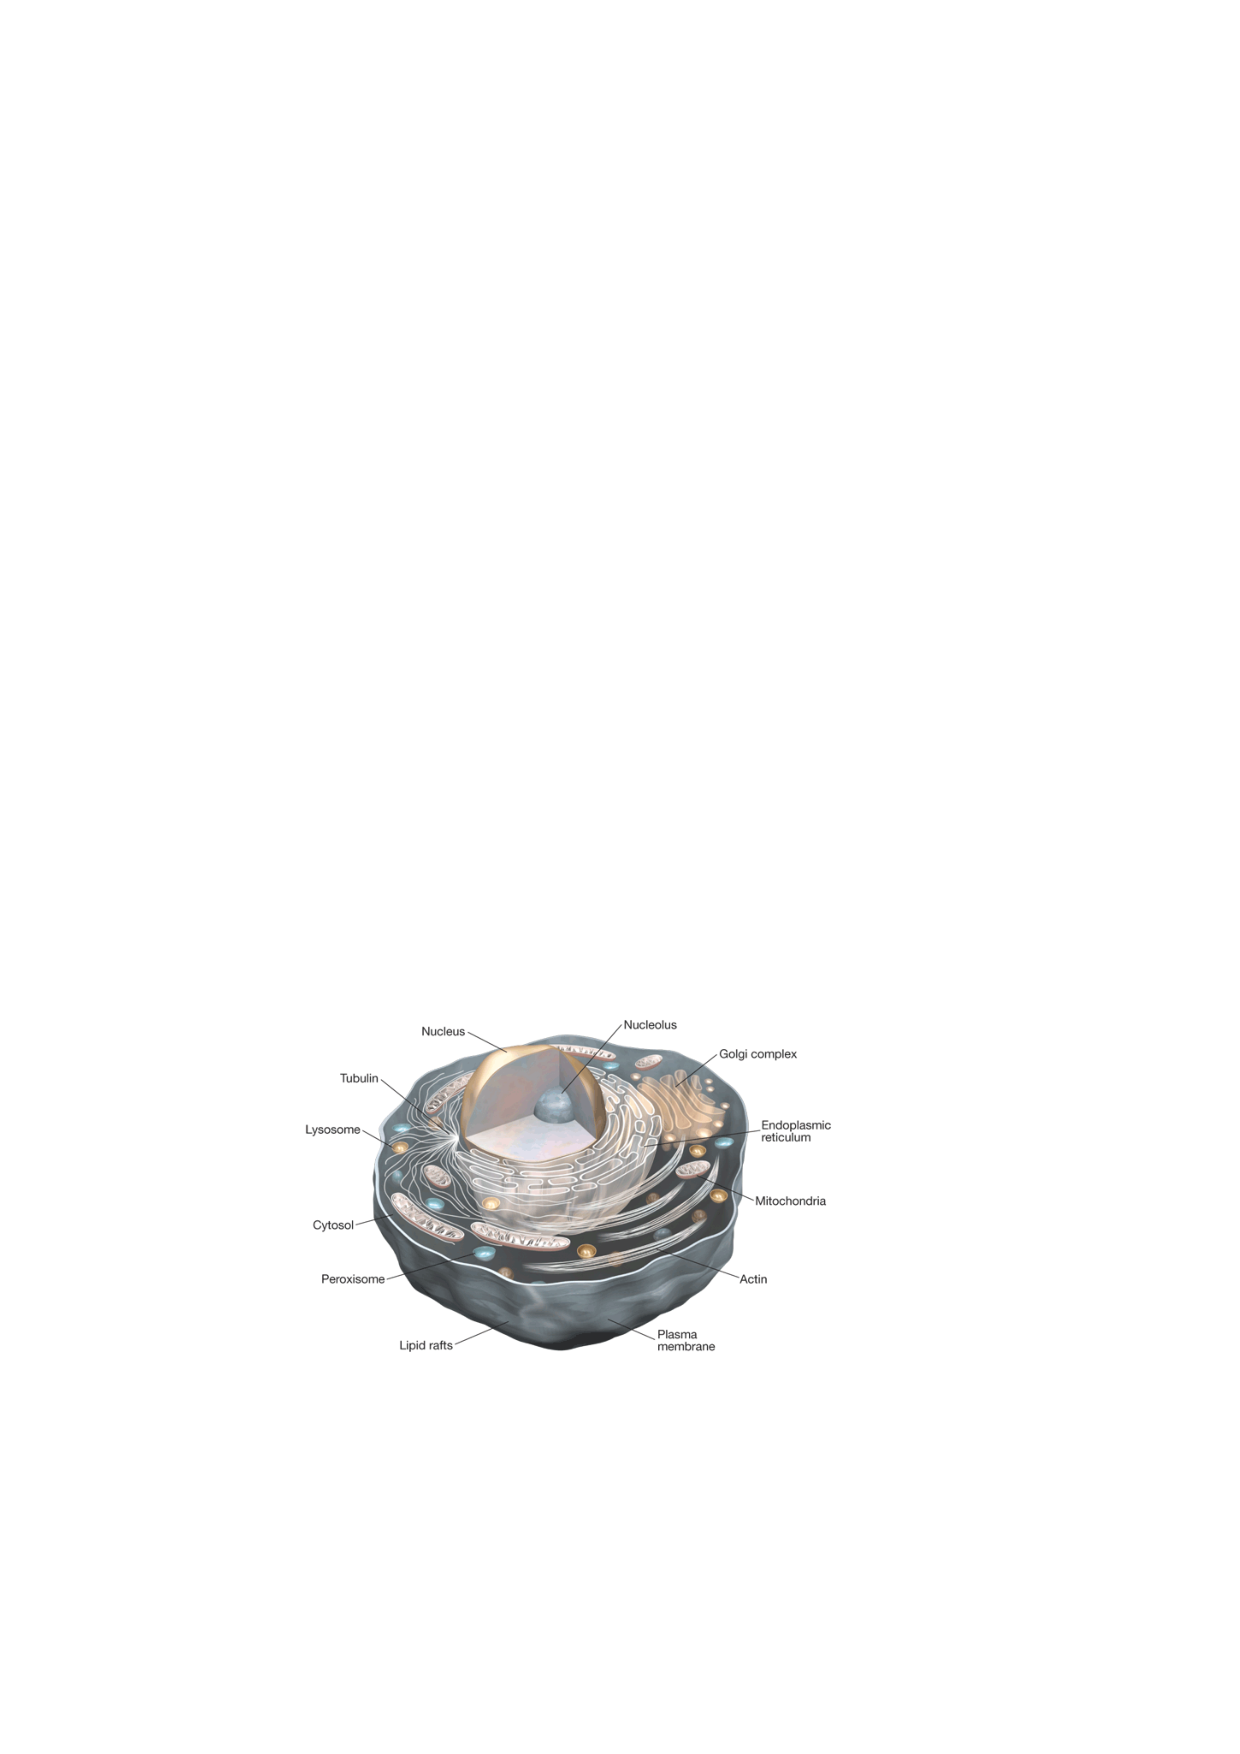
\includegraphics[width=\columnwidth]{\MemBio /Pics/CellParts}
\caption{
شکل طراحی شده از سلول پستانداران که غشا و اعضای سلول را نشان می‌دهد
\cite{CellParts}.
}
\label{fig:cellparts}
\end{center}
\end{figure}

مولکول‌ها مهم‌ترین نقش غشاهای زیستی ایجاد یک دیوار یا مانع برای مشخص کردن مرز داخل و خارج سلول است که نیاز اولیه‌ی وجود حیات به حساب می‌آید
\cite{Boyle2008Biology}.
 علاوه بر در-بر-گرفتنِ تمام اعضای یک سلول، در سلول‌های هسته‌دار، غشای هسته اوگان‌های خیلی مهم سلول را نیز در خود جای داده و محافظت می‌کند (شکل
\ref{fig:cellparts}).
 به عنوان مرز سلول با دنیای خارج، غشا نقش مهمی در مدیریتِ نقل و انتقال مواد بین سلول و محیط پرامون دارد. درون غشا پروتئین‌ها، لیگاند‌ها\LTRfootnote{ligand},
و مولکول‌های درشت زیادی وجود دارد که در طیف‌ گسترده‌ای از فرآیندها نقش دارند. برای مثال غشا نقل و انتقال یون‌ها به درون و خارج سلول را از طریق کانال‌های پروتئینی مدیریت می‌کند
\cite{NEHER1976ProteinChannel}،
نسبت به تغییر فشار اُسمزی محیط واکنش نشان می‌دهد
\cite{Perozo2006Osmotic,Vasquez2009Osmotic,Haswell2011Osmotic}،
و همچنین در ساز و کار‌های بزرگ مقیاس مانند تقسیم سلولی، حرکت و جابجایی سلول، و چسبیدن به سطوح نقش دارد.


غشای سلول در خیلی از مسائل مهم پزشکی نیز مطرح می‌شود، مانند نقش آن در انتقال پالس الکتریکی در سلول‌های عصبی هنگام بیهوشی عمومی 
\cite{BioMemBook2007}.
همچنین بیشتر تلاش صنعت داروسازی طراحی داروی مناسب برای اتصال به پروتئین‌های روی سطح غشاست. به طور تقریبی، یک سوم پروتئین‌های درون بدن در غشای سلول قرار دارند که  مورد هدف ۶۰ درصد از داروی‌های موجود در بازار هستند
\cite{DrugDelivery2007}.
 دانش یافته شده از مطالعه‌ی غشا در تکنولوژی‌های مدرن مانند بسته‌بندی و انتقال دارو
\cite{Torchilin2006Drugdelivery}،
ایجاد اتاقک‌های کوچک برای انجام واکنش‌های شیمیایی
\cite{Karlsson2001MemChamber}،
 و ساخت حس‌گرهای زیستی (ترکیب دستگاه‌های الکتریکی با غشا) کاربرد دارد
\cite{MemeElctronics2012}.
